\subsection{Database}
Una parte fondamentale del progetto è il database, in quanto è usato per contenere le informazioni che veranno poi usate dal sito.\\
È stato pensato di creare un database con la funzione di contenere tutti i dati relativi ai prodotti in vendita compresi i voti e i commenti, agli eventi a cui è possibile partecipare e i dati degli utenti registrati.\\
Come si può vedere dalla \emph{Figura \ref{Fig:schemadb}}, le tabelle sono sei:
\begin{itemize}
		\item \textbf{Eventi:} contiene il titolo, la data, il luogo e la descrizione degli eventi a cui sarà possibile partecipare
		\item \textbf{Categoria:} contiene il nome delle categorie
		\item \textbf{Prodotti:} contiene il nome, l'immagine, gli ingredienti e la descrizione dei prodotti venduti
		\item \textbf{Utenti:} contiene l'username e la password degli utenti iscritti. Inoltre si verifica se l'utente è un admin.
        \item \textbf{Voti:} contiene i voti degli utenti
        \item \textbf{Commenti:} contiene i commenti degli utenti
\end{itemize}
\begin{figure}[!h]
	\centering	% L'immagine aggiornata è presente nel branch Main
	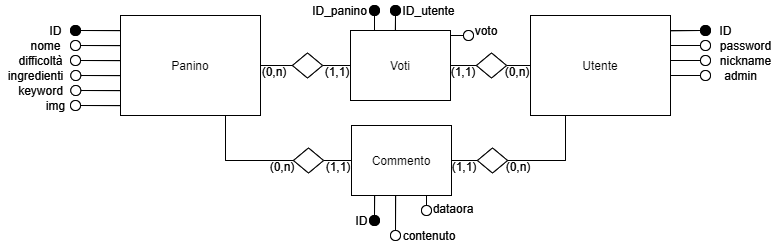
\includegraphics[width=0.7\linewidth]{../database/DiagrammaER.png}\\
    \caption{Schema concettuale database}
	\label{Fig:schemadb}
\end{figure}
Il database viene interrogato da \emph{PHP} quando bisogna utilizzare o richiamare le informazioni.
Le pagine: \emph{Eventi}, \emph{I nostri Burger}, \emph{Panino} sono riempite dinamicamente tramite chiamata \emph{PHP}.\\
Come spiegato nella sezione \emph{Analisi}, esistono due tipi di utenti: \emph{utente generico} e \emph{amministratore}. Nel database viene utilizzato un booleano per differenziare le due tipologie.\\ 